%!TEX root = ../Main.tex
This section will mark the conclusion of the preliminary work done in \cref{theorysec,hamilsec,greensec}. All the functions producing on-site Hamiltonians, hopping matrices, full Hamiltonians, band structures as well as self-energy and Green's functions by recursion, will be used to get the transmission through the material.\\
\subsection{Left-right device geometry, rate matrices and spectral functions}
First of all a sentence as to what transmission is: Transmission is the probability of an electron being transported trough a specific region for a specific range of energies and thus how the region affects the overall current flow of electrons through the system as a whole. Below is an equation stating it formally
\begin{align}\label{transformal}
	P(t)_{mn} = \left|\mel{m}{e^{i\vb{H}t/\hbar}}{n}\right|^2
\end{align}
where \(m,n\) is the density of states in each side of the region of interest (states going in/out) and \(e^{i\vb{H}t/\hbar}\) is the solution to the Green's function.\\
To give an overview and explain the different concepts of transmission this section will rely heavily on \cref{systemillu} where all the different parts of the system have been translated from the actual material into mathematical
formalism in the shape of matrices.
\begin{figure}
	\centering
	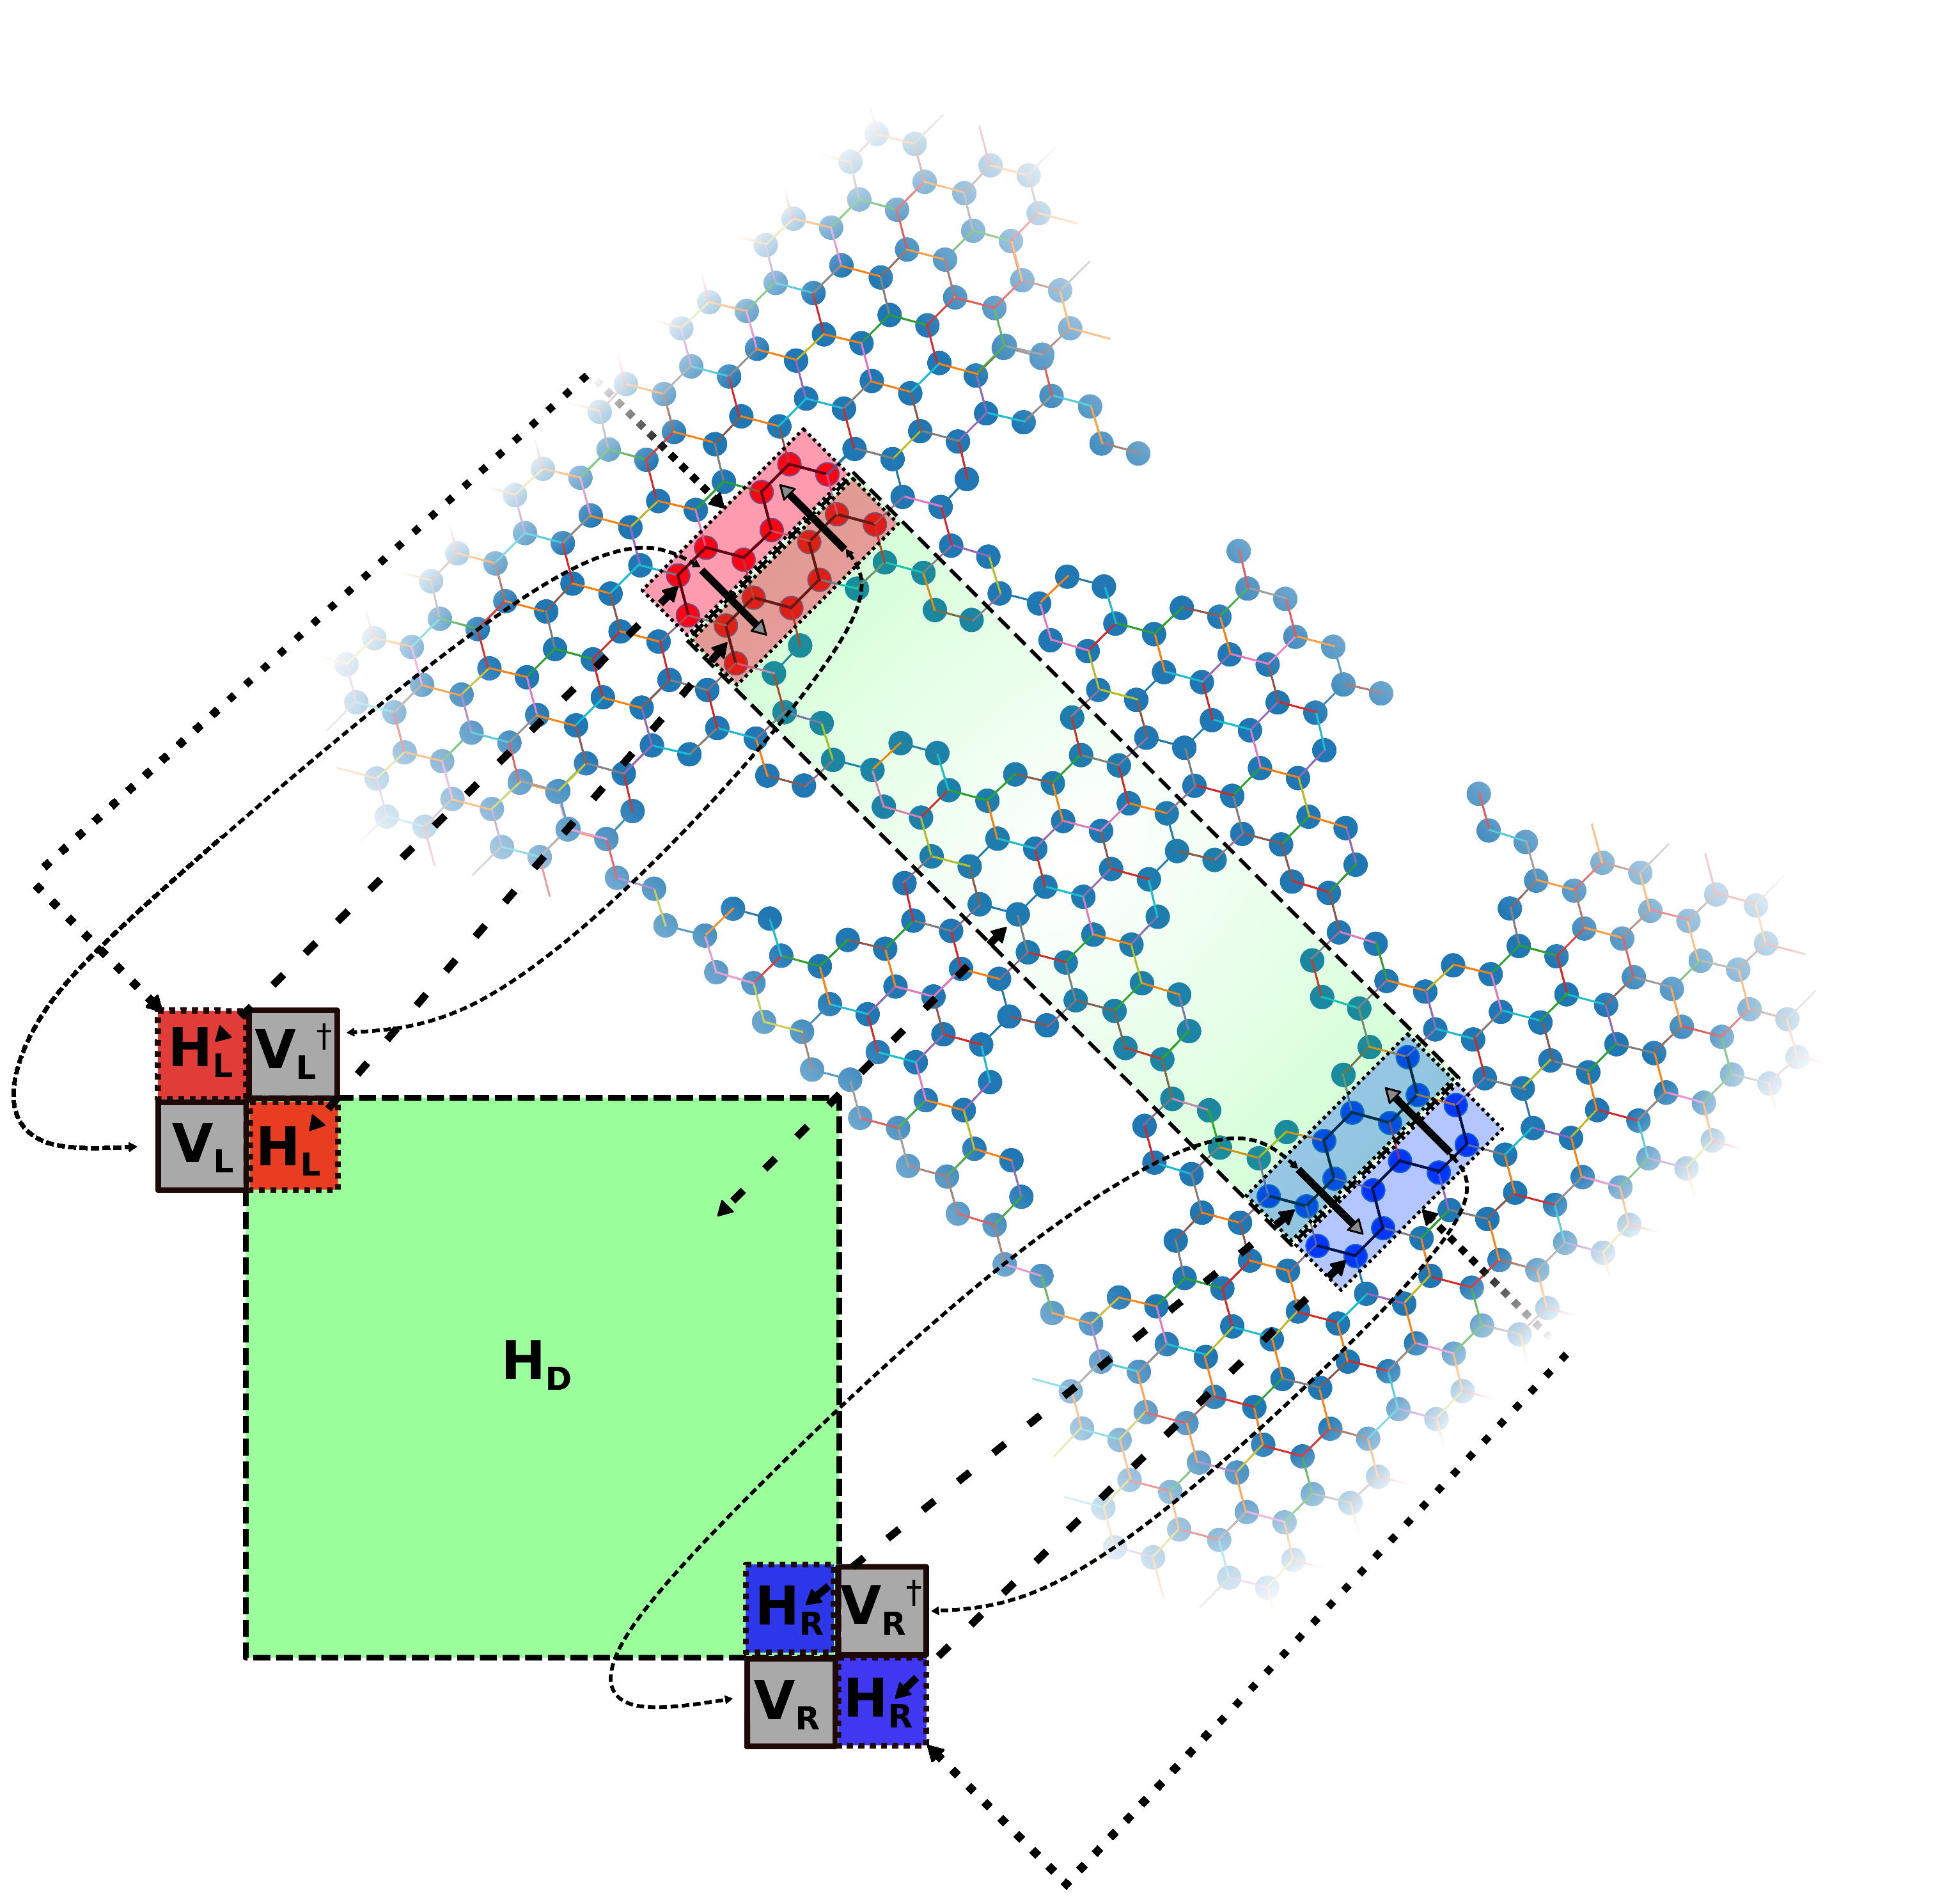
\includegraphics[width=0.9\textwidth]{Figures/illu.eps}
	\caption{Illustration showing how the different parts of the system are translated into matrix blocks in NPG. The green box is the unit cell of the device with the Hamiltonian \(\textbf{H}_D\). It includes one red and blue box which themselves are unit cells of the left and right contacts and have the Hamiltonians \(\textbf{H}_L,\ \textbf{H}_R\). The two other unit cells lying outside the device region represents what could be an infinite contact region reducible by recursion. Finally the two fat black arrows (not dotted) on each side of the device represents the hopping between the device- and contact region. Note that the direction of hopping corresponds to a specific hopping matrix. F.ex. left-to-right is the ordinary hopping matrix (\(\vb{V}\)) while right-to-left is its conjugate (\(\vb{V}^{\dagger}\)) (for both left and right side of the device).}
	\label{systemillu}
\end{figure}
The first and central piece is the so-called "Device Region" with the on-site Hamiltonian \(\vb{H}_D\) (Green area in \cref{systemillu}). The device region contains at least one central unit cell as well as a "left" and "right" unit cell (Red and blue area in \cref{systemillu}). The left and right unit cells represent the contact region of the device i.e. the two parts that connects to the rest of the system/molecule. They have on-site Hamiltonians \(\vb{H}_L,\vb{H}_R\) and they interact with rest of the system via hopping matrices \(\vb{V}_{L,R},\vb{V}^{\dagger}_{L,R}\). As \(\textbf{H}_D\) contains \(\textbf{H}_{L,R}\) they can be picked out of \(\textbf{H}_D,\)  without further calculation (See \cref{systemillu}) once the \(\vb{H}_D\) has been calculated. The cells next to the contact region can be reduced into a single Hamiltonian by recursion to have same dimension as \(\vb{H}_{L,R}\). Note that \(\vb{H}_{L,R}\) need not be the same dimensions.
Related to \(\vb{H}_{L,R}\) is the left and right self-energies \(\vb{\Sigma}_{L,R}\) and on-site Green's matrices \(\vb{g}_L\), \(\vb{g}_R\). These can be obtained using the theory and developed methods from \cref{greensec}. However the aim is to obtain the Green's matrix for the device region, \(\vb{G}_D\), as it is the one needed to fully describe the transmission in the region of interest. In other words, propagation of the states in the green area in \cref{systemillu}. To obtain it, one simply has to keep in mind that the effective coupling of the device region to the rest of the system is determined by the two contact regions (\(\vb{H}_{L,R}\)) and thus the correction to the device Green's functions will be determined by the self-energy of those contact regions. So the Green's matrix will be given by the same equation as \cref{Greenssolved} but with a self-energy correction going left ad right:
\begin{align}\label{devicegreenseq}
	\vb{G}_D & = [\vb{1}(E+i\eta) - \vb{H}_D - \vb{\Sigma}_L(E) - \vb{\Sigma}_R(E)]^{-1}
\end{align}
Looking back at \cref{transformal} the Green's function needed has been obtained, but what about the states going in and out of the device region \(\bra{m}\ \text{and}\ \ket{n}\)? As states travel, their corresponding self-energies change in time. Rate operators \(\vb{\Gamma}\) are defined as the change in imaginary self-energy. They describe the 'rate' by which the self-energies of the states moving in and out, change in time. The rate matrices are given by
\begin{align}\label{rateeq}
	\vb{\Gamma}_{L,R} = i(\vb{\Sigma}_{L,R} - \vb{\Sigma}^{\dagger}_{L,R})
\end{align}
Similarly the change in the imaginary Green's matrix is defined as
\begin{align}
	\vb{A} & = i(\vb{G}-\vb{G}^{\dagger})                                                                                  \\
	       & = i(\vb{G}^{\dagger}\left[\vb{G}^{\dagger}-\vb{G}\right]^{-1}\vb{G})\nonumber                                 \\
	       & = i(\vb{G}^{\dagger}[E-\vb{H}^{\dagger}-\vb{\Sigma}^{\dagger} - (E -\vb{H}-\vb{\Sigma})]^{-1}\vb{G})\nonumber \\
	       & =i(\vb{G}^{\dagger}[-\vb{\Sigma}^{\dagger}+\vb{\Sigma}]^{-1}\vb{G})\nonumber                                  \\
	       & =i(\vb{G}^{\dagger}\vb{\Gamma}\vb{G})
\end{align}
Here it have been utilised that the Green's matrix is symmetric in time (\(\vb{G}=\vb{G}^{T}\), \(\vb{G}^{T}\vb{G}=\vb{I}\), \(\vb{G}^{T}=\vb{G}^{-1}\)) as well as the fact that \(\vb{G} = [z\vb{1}-\vb{H}-\vb{\Sigma}]^{-1}\). Additionally the Hamiltonians cancel out as they are unitary.
The definition of \(\vb{A}\) is that it is a \textit{spectral function}. It is the change of the imaginary Green's functions. As seen in the equations above it can be described by the Green's matrix and the rate matrix. From the previous sections it is know that the imaginary part of the Green's functions represent the LDOS. The spectral function is thus describing the density of states, changing by the rate \(\vb{\Gamma}\). The spectral function can also be described in 'left/right' terminology as
\begin{align}
	\vb{A}_{L,R} = \vb{G}_{D}^{\dagger}\vb{\Gamma}_{L,R}\vb{G}_{D}
\end{align}
Taking the left spectral function as an example, it represents the density of states of a wave coming from the left entering the device. To describe how the density of states pass through the device region from left-to-right or right-to-left one just have to multiply the spectral function by the appropriate rate matrix. Again using the left spectral function as an example
\begin{align}\label{spectraltrace}
	\text{Tr}[\vb{A}_L\vb{\Gamma}_R]=\text{Tr}[\vb{G}_{D}^{\dagger}\vb{\Gamma}_{L}\vb{G}_{D}\vb{\Gamma}_R]
\end{align}
Here the trace of the product is taken as all states besides the one in the left contact region are zero. This corresponds to the density of states coming from the left, which then pass on through the right electrode by the rate \(\vb{\Gamma}_R(E)\). Additionally the trace is cyclic so
\begin{align}\label{lilletrans}
	\text{Tr}[\vb{A}_L\vb{\Gamma}_R]=\text{Tr}[\vb{A}_R\vb{\Gamma}_L]
\end{align}
This ultimately leads to transmission because transmission is in essence an expression of how much of the density of states passes trough the device and as explained, \cref{spectraltrace} is exactly the density of states, coming from the left (or right) and then passes through the right (left) by rate \(\vb{\Gamma}_{L,R}(E)\). So using the Green's function, left/right self-energies as well as the left/right rate matrices, the transmission, as a function of energy, can be obtained via the following equation:
\begin{align}
	T(E) = \text{Tr}[\vb{\Gamma}_R\vb{G}_D\vb{\Gamma}_L\vb{G}_D^{\dagger}](E)
	\label{transeq}
\end{align}
\subsection{Transmission in 1D}
Again the developed routine in this section will be used on the simple system (\cref{inlinepointplot}) as an example and in order to make sure that the obtained results are as expected. First thing is to define the device in the same manner as \cref{systemillu} so that the device Hamiltonian \(\textbf{H}_D\) can be obtained through the already defined function \textit{Onsite}. The left and right Hamiltonian \(\textbf{H}_{L,R}\) are thus picked out as described earlier. An implementation has been made to the script to allow the user to see the left and right contact cells graphically as red and blue marked atom indices in the plot of the unit cell (See \cref{inlinepointplot}).
This allows the user to get an overview of dimensions of \(\vb{H}_{L,R}\). The hop matrices are then defined using the \textit{Hop} function. This requires at least a five cell system as shown in \cref{2DHammil}.
\begin{figure}[ht]
	\centering
	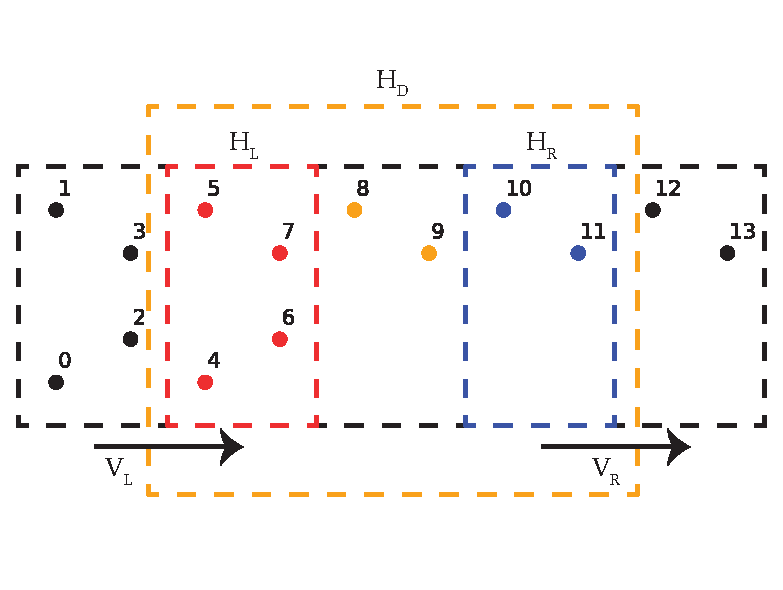
\includegraphics[width=.7\textwidth]{Figures/2DHam.eps}
	\caption{All onsite on offsite hop elements and contact Hamiltonians can be extracted from the matrix produced by \textit{PeriodicHamiltonian} because of the 5-cell setup. \(H_D\) is the device Hamiltonian, \(H_L\) and \(H_R\) are contact Hamiltonians; \(V_L\) and \(V_R\) are hopping matrices (here shown as arrows).}
	\label{2DHammil}
\end{figure}
The device itself consists of two contacts and everything in between. An extra cell on each contact represent the semi-infinite chain.\newline
Now that the Hamiltonians and hop matrices are found, the developed \textit{EnergyRecursion} function is used to obtain the device Green's matrix. This function is a more elaborate version of the earlier mentioned \textit{RecursionRoutine} and it takes \(\vb{H}_D,\vb{H}_L,\vb{H}_R,\vb{V}_L,\vb{V}_R\), a range of energies and \(\eta\) as inputs. As these matrices are sparse, it is memory efficient to convert them to compressed sparse row matrices as shown in \cref{sparse}. This is, however, a trade-off as numerical computations will take more time.
\im{Listings/Functions.py}{199}{203}
\vspace{-.5\baselineskip}
\captionof{listing}{By using SciPy, \textit{EnergyRecursion} converts all matrices to the more memory efficient ``Compressed Sparse Row matrix''.\label{sparse}}\vspace{\baselineskip}
The next step is to calculate the self-energies for the left and right cells (\(\vb{\Sigma}_{L,R}\)) and the Green's functions for the left and right cells (\(\vb{g}_{L,R}\)) using the \textit{RecursionRoutine} as shown in \cref{ERR}.
\im{Listings/Functions.py}{210}{212}
\vspace{-.5\baselineskip}
\captionof{listing}{The Green's functions and self-energies are calculated, first from left and then from right. This is done for each energy in a selected energy range (\textit{En})\label{ERR}}\vspace{\baselineskip}
The device Green's function \(\textbf{G}_D\) as well as the left and right rate matrices \(\vb{\Gamma}_{L,R}\), are then calculated using \cref{devicegreenseq,rateeq}, as shown in \cref{GGG}.
\im{Listings/Functions.py}{225}{228}
\vspace{-.5\baselineskip}
\captionof{listing}{The device' Green's functions and the left and right rate matrices are calculated in \textit{EnergyRecursion} as shown.\label{GGG}}\vspace{\baselineskip}
The output of the \textit{EnergyRecursion} function is the two rate matrices \(\vb{\Gamma}_{L/R}\) as well as the device Green's function \(\vb{G}_D\) and as per \cref{transeq} the matrices needed for transmission have been obtained. As seen in \cref{transfunc} the function \textit{Transmission} simply carries out the matrix product and subsequent trace of the matrices resulting from \textit{EnergyRecursion} and outputs a range of transmission probabilities which is then plotted against an energy range. Do mind that this is still just 1D in the sense that the transmission only moves in one direction. A plot of the transmission for the simple 1D system (the one in \cref{inlinepointplot}) can be seen in \cref{Transsimple}.
\im{Listings/Functions.py}{240}{243}
\vspace{-.5\baselineskip}
\captionof{listing}{Code showing how the transmission probabilities are calculated. Taking rate matrices, device Green's function and a range of energies as inputs, it takes the trace of the matrix product for a range of energies as in \cref{transeq}. \label{transfunc}}\vspace{\baselineskip}
The transmission-function also transform the transmission and Green's function to normal ``dense'' matrices, as these are no longer excessively large, nor sparse.
\begin{figure}[ht]
	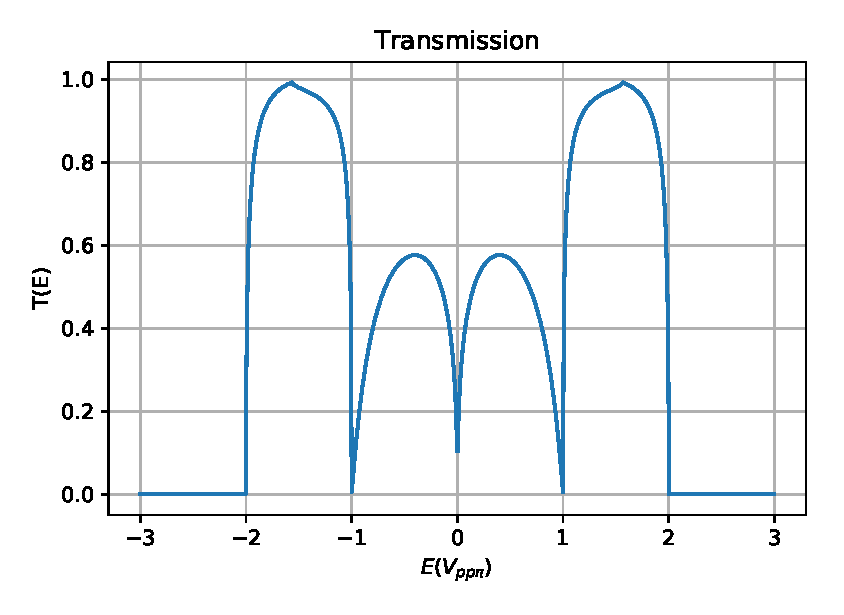
\includegraphics[width=0.45\textwidth]{Figures/BetaTE.eps}
	\caption{Figure showing the resulting transmission through the simple system}\label{Transsimple}
\end{figure}
\subsection{Development of transmission to 2D}\label{trans2d}
Now that transmission for a semi-infinite chain can be found, the last step is to expand the code for cells stacked on top of the chain. Such a configuration will constitute a sheet of repeated unit cell structures as shown in \cref{2DTranssys}.
\begin{figure}[ht]
	\centering
	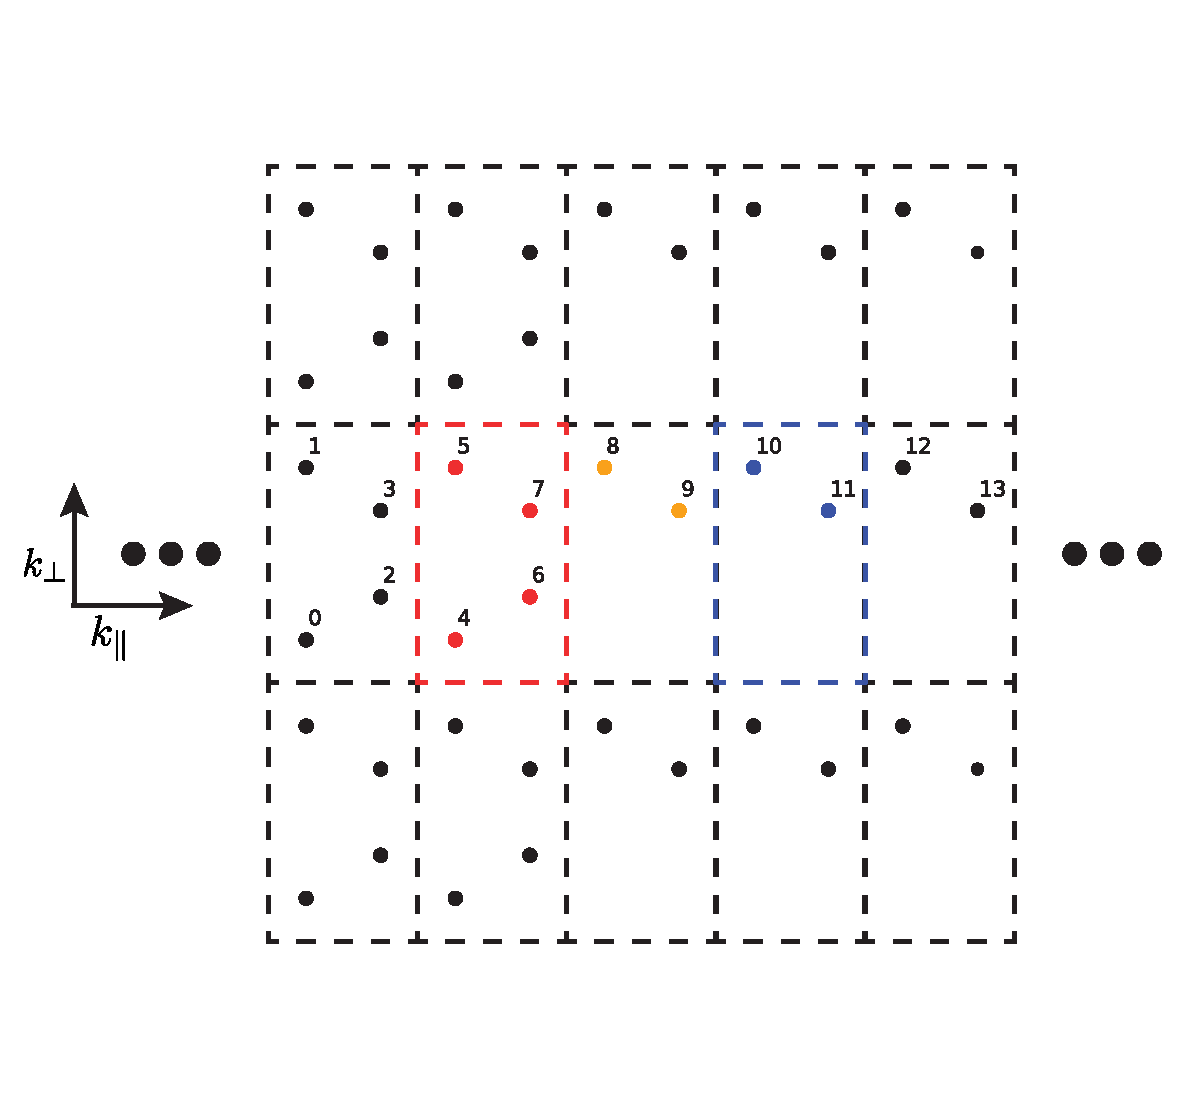
\includegraphics[width=.7\textwidth]{Figures/2DTrans.eps}
	\caption{The simple system repeated in 2D. The k-points perpendicular to the transport direction are shifted with a Bloch phase. This practically packs the system to just one row of cells, which in turn is dealt with using the \textit{EnergyRecursion} routine.}
	\label{2DTranssys}
\end{figure}
Because of its periodicity, the structure is, as before, described in reciprocal space. The semi-infinite chain runs along \(k_{\|}\), with the chains stacked along \(k_{\perp}\).
Before describing this system there are two considerations: Firstly the range of \textit{k}-points in \(k_{\perp}\) exists between \(-\pi\) and \(\pi\). Secondly these are periodic boundaries. When an electron exits at the top of the chain, it reappears at the bottom with a Bloch phase shift.
Now the method is to pick a range of perpendicular \textit{k}-points of interest and then the idea is to construct a Hamiltonian for the 1D chain, located at that point. This Hamiltonian contains hop elements in the perpendicular direction, accounting for transport perpendicular to the semi-infinite chain. The recursion routine then calculates Green's functions and transmission. The Hamiltonian is constructed using the function \textit{PeriodicHamiltonian}. This function uses the equation:
\begin{align}
	\vb{H} = \vb{h} + \vb{V}\me^{ik_{\perp}} + \vb{V}^{\dagger}\me^{i-k_{\perp}}\label{PBHEQ}
\end{align}
The equation is applied in \cref{PBH}.
\im{Listings/Functions.py}{250}{253}
\vspace{-.5\baselineskip}
\captionof{listing}{The function calculating the periodic Hamiltonian for a given \textit{k}-point using \cref{PBHEQ}.}{\label{PBH}}\vspace{\baselineskip}
As seen in \cref{PBH}, the onsite and hop matrices are calculated in the usual way but for all of the atoms in the 5 cells. In order to understand why, first consider \cref{2DHammil}.
Because of the 5-cell setup it is possible to extract all hop elements and Hamiltonians from the output matrix of \textit{PeriodicHamiltonian}. The contact Hamiltonians exists in the ends of the diagonal and some off diagonal elements contains the hop elements. These are extracted in the 2D transmission routine as shown in \cref{MatrixEx}.
\im{Listings/NPGTransmission.py}{39}{47}
\vspace{-.5\baselineskip}
\captionof{listing}{All required matrices for the recursion routine can be picked from the periodic Hamiltonian.}{\label{MatrixEx}}\vspace{\baselineskip}
To get the transmission in 2D the function \textit{PeriodicHamiltonian} is nested in a for loop, looping over transverse k-points. Still within the loop the \textit{EnergyRecursion} is used to get the device Greens function, and left/right rate matrices. Lastly the transmission is calculated with the function \textit{Transmission} using \cref{transeq}.
Plots for transmission per k-point will be shown for NPG in \cref{CompTB}.
\subsection{Summary of developed scripts}
\begin{figure}[ht]
	\centering
	\includegraphics[width=\textwidth]{Figures/Flowchart.eps}
	\caption{Flowchart depicting the routines run in Python. SISL is used to import the geometry. Afterwards the coordinates are either used for band structure plots or for transmission plots. For the band structures, a Hamiltonian at each desired k-point is generated and diagonalised in order to get the eigen energies. These energies are then plotted. With transmission, a periodic Hamiltonian at various transverse k-points are generated and reduced to self-energies in the transport direction (using the recursion algorithm). The self-energies and the Green's functions retrieved here are then multiplied as to get the transmission.}
	\label{Flowchart}
\end{figure}
The final algorithm is shown in \cref{Flowchart}. It is laid our here:
\begin{enumerate}
	\item Import geometry and unit vectors with SISL.
	\item For band structure plots
	      \begin{enumerate}
		      \item Find the Hamiltonian described in \cref{hamilsec}
		      \item Calculate the eigen energies, iterating over the desired k-points.
		      \item Plot the gathered k-points.
	      \end{enumerate}
	\item For transmission plots.
	      \begin{enumerate}
		      \item Hamiltonian at a specific \(k_{\perp}\)-point is generated.
		      \item Iterating over the energies, the (at least 5-cell) system is reduced using the recursion routine.
		      \item Iterating over the energies, the self-energies and Green's functions are used to calculate transmission.
		      \item Transmission, Green's functions and LDOS are plotted.
	      \end{enumerate}
\end{enumerate}
\subsection{Comparing tight-binding with DFT and TBtrans for transmission and band structure calculations in NPG}\label{CompTB}
All the scripts necessary for calculation have been developed and they can now be used on a system of NPG.
The following results are based on this structure similar to that of \cref{introGraphic}. Firstly the band structure obtained using the script described in \cref{FullHam} is shown together with  band plots obtained from DTF and TBtrans calculations.
\begin{figure}[H]
	\centering
	\begin{subfigure}[t]{0.45\textwidth}
		\centering
		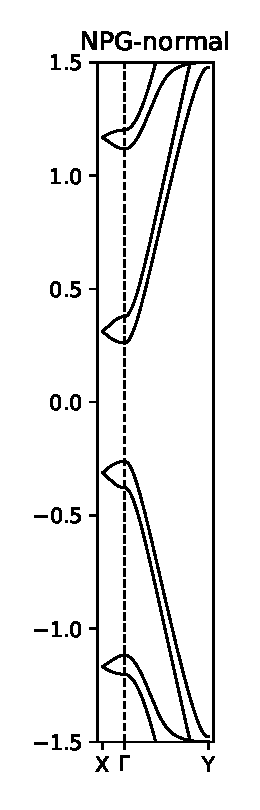
\includegraphics[width=0.5\textwidth]{Figures/NPG-normalBandstructures.eps}
		\caption{Figure showing the band structure for NPG with normal bridges obtained with the script described in \cref{FullHam}}
		\label{bsscript}
	\end{subfigure}
	~  %add desired spacing between images, e. g. ~, \quad, \qquad, \hfill etc.
	%(or a blank line to force the subfigure onto a new line)
	\begin{subfigure}[t]{0.45\textwidth}
		\centering
		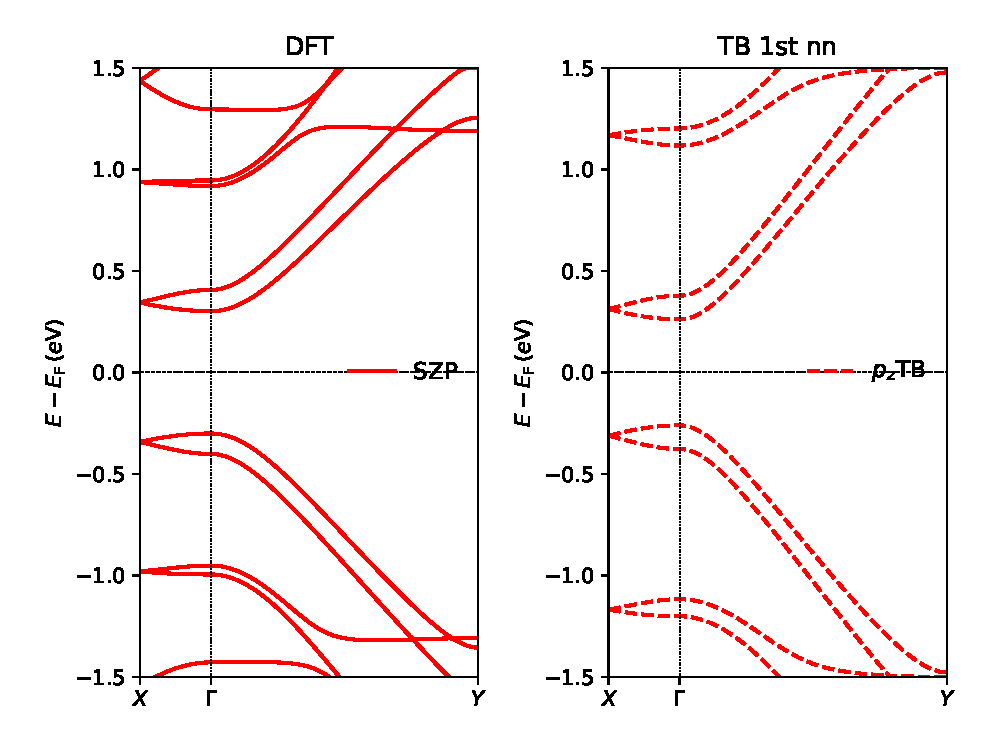
\includegraphics[width=\textwidth]{Figures/bands.eps}
		\caption{Figure showing the bands structures obtained from DFT and TBtrans calculations.}
		\label{bsdfttbt}
	\end{subfigure}
	\caption{Figure showing how the band plots compare for DFT, TBtrans and the developed script.}\label{bandcompare}
\end{figure}
The band plot obtained in \cref{bsscript} shows almost 1-to-1 correspondence with the plot obtained using TBtrans \cref{bsdfttbt} (right) and is also very similar to the plot obtained from DFT \cref{bsdfttbt} (left), proving that the script is capable of creating band structures for NPG-systems. Next is a comparison of the transmission in NPG for different k-points in reciprocal space. The plots are made for transmission through NPG in real space (x-direction) for each three different k-points in the reciprocal space (\(\dfrac{1}{y}\)-direction). The three k-points are \(0,\ \dfrac{\pi}{2},\ \pi\). Additionally an average over these k-points is plotted as well. In \cref{transmissionplots} transmission plots obtained with the script described in \cref{trans2d} is compared with transmission plot obtained through DTF, using the same k-points.
\begin{figure}[H]
	\centering
	\begin{subfigure}[b]{\textwidth}
		\centering
		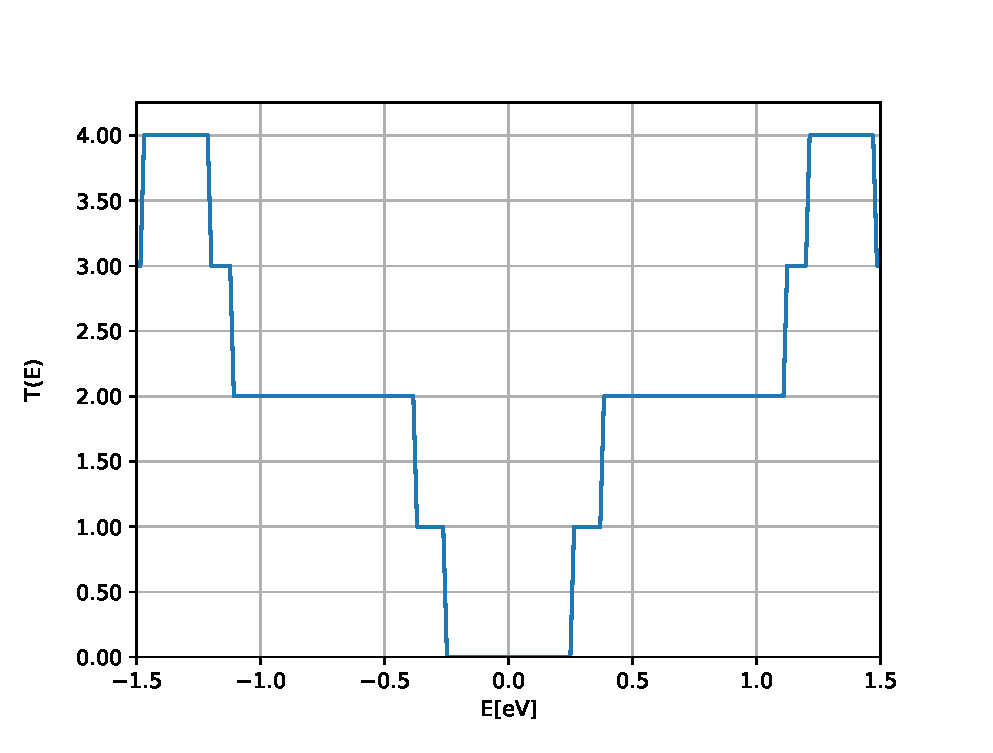
\includegraphics[width=0.38\textwidth]{Figures/NPGNormal_0.eps}
		\qquad
		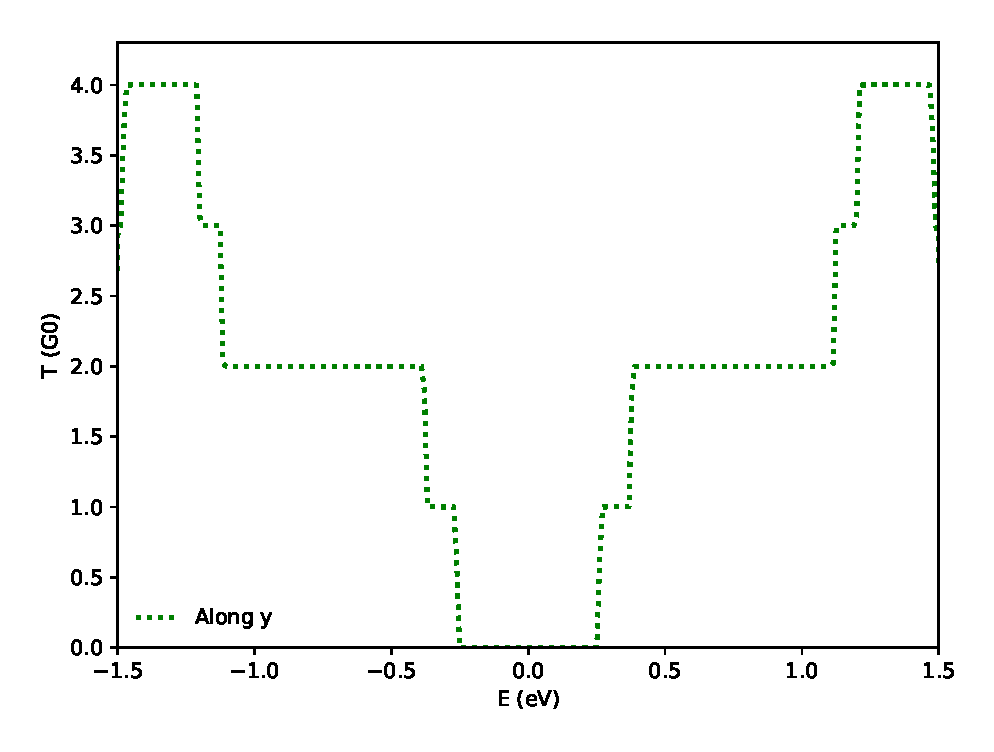
\includegraphics[width=0.35\textwidth]{Figures/txy_0.eps}
		\caption{Transverse k-point 0}
		\label{pizero}
	\end{subfigure}
	\vskip
	\begin{subfigure}[b]{\textwidth}
		\centering
		\includegraphics[width=0.38\textwidth]{Figures/NPGNormal_pi-half.eps}
		\qquad
		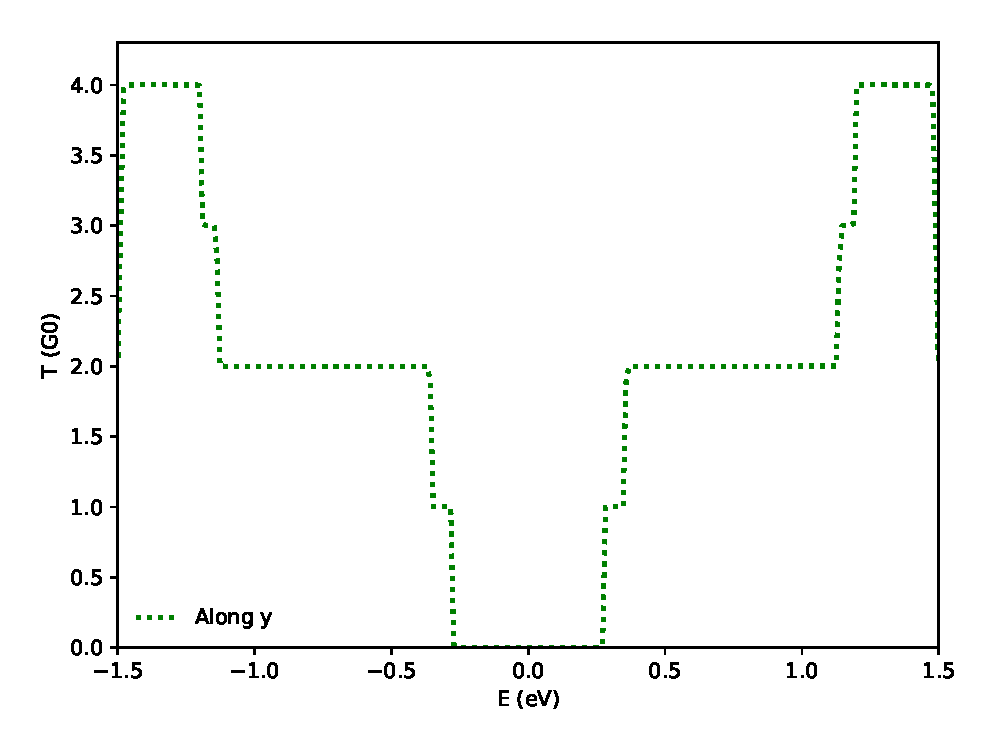
\includegraphics[width=0.35\textwidth]{Figures/txy_pi-half.eps}
		\caption{Transverse k-point \(\dfrac{\pi}{2}\)}
		\label{pihalf}
	\end{subfigure}
	\vskip
	\begin{subfigure}[b]{\textwidth}
		\centering
		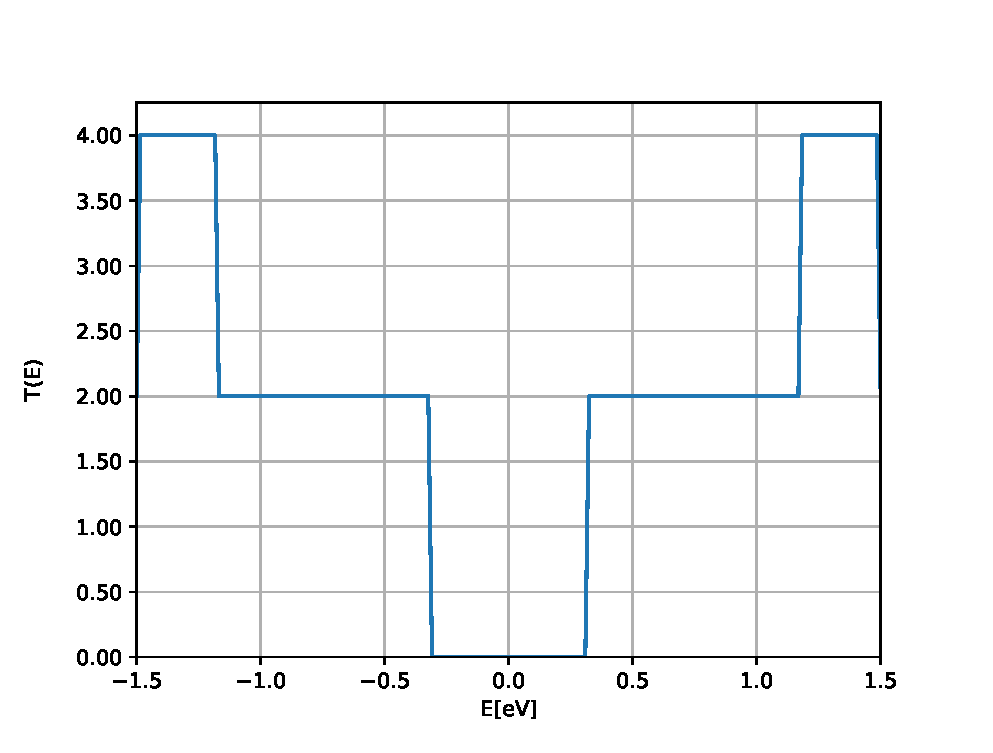
\includegraphics[width=0.38\textwidth]{Figures/NPGNormal_pi.eps}
		\qquad
		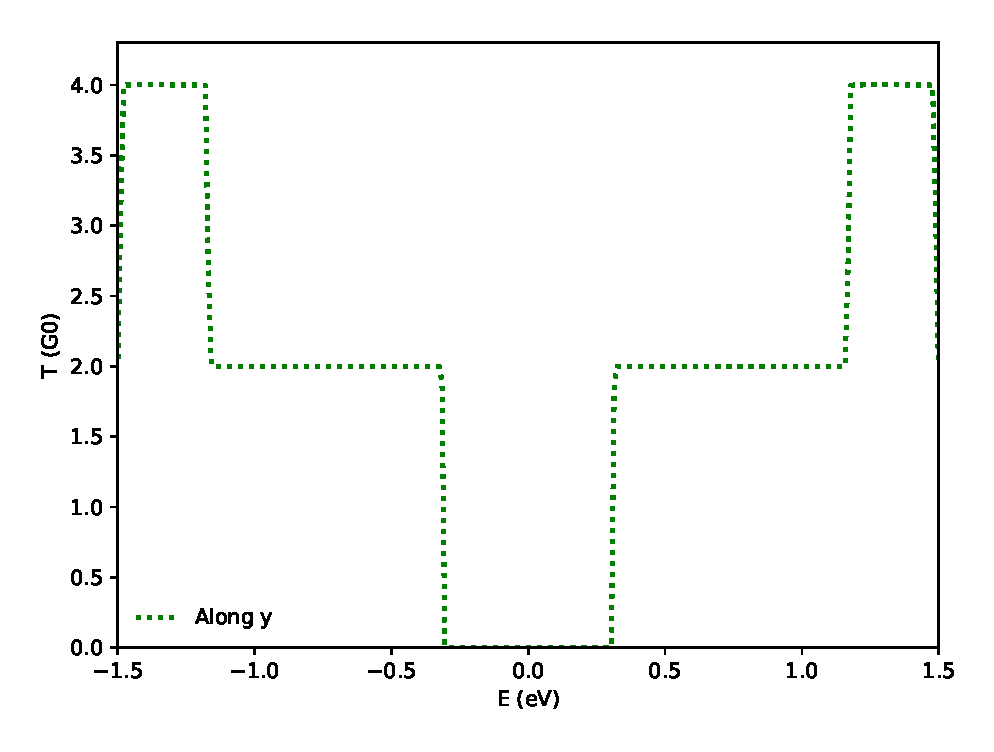
\includegraphics[width=0.35\textwidth]{Figures/txy_pi.eps}
		\caption{Transverse k-point \(\pi\)}
		\label{pi}
	\end{subfigure}
	\vskip
	\begin{subfigure}[b]{\textwidth}
		\centering
		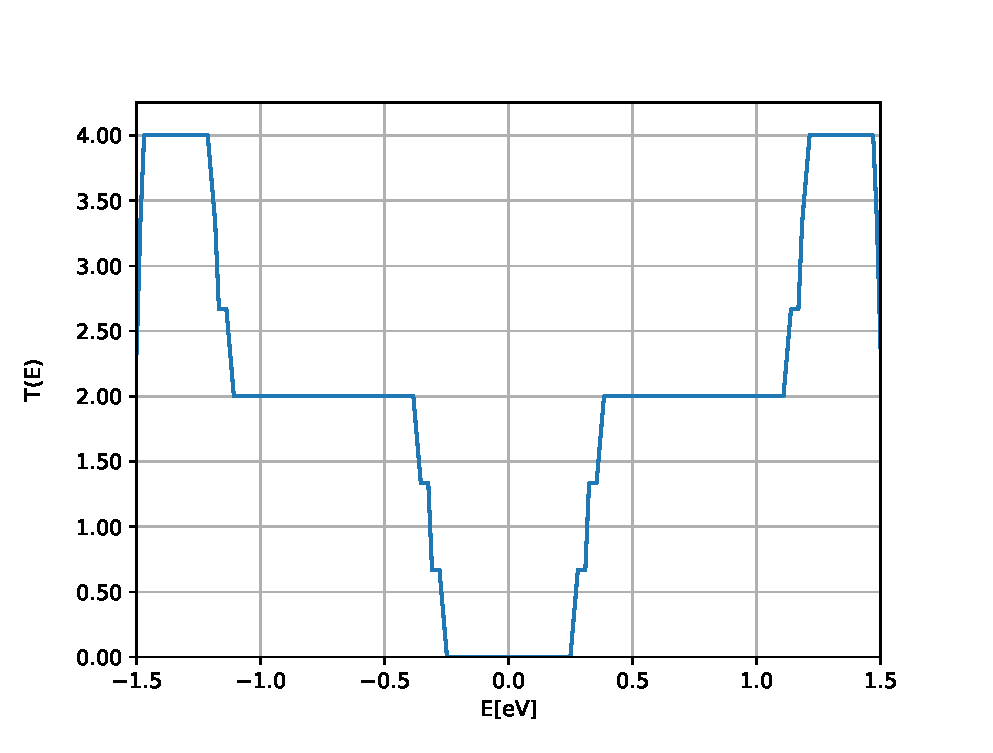
\includegraphics[width=0.38\textwidth]{Figures/NPGNormal_AVER.eps}
		\qquad
		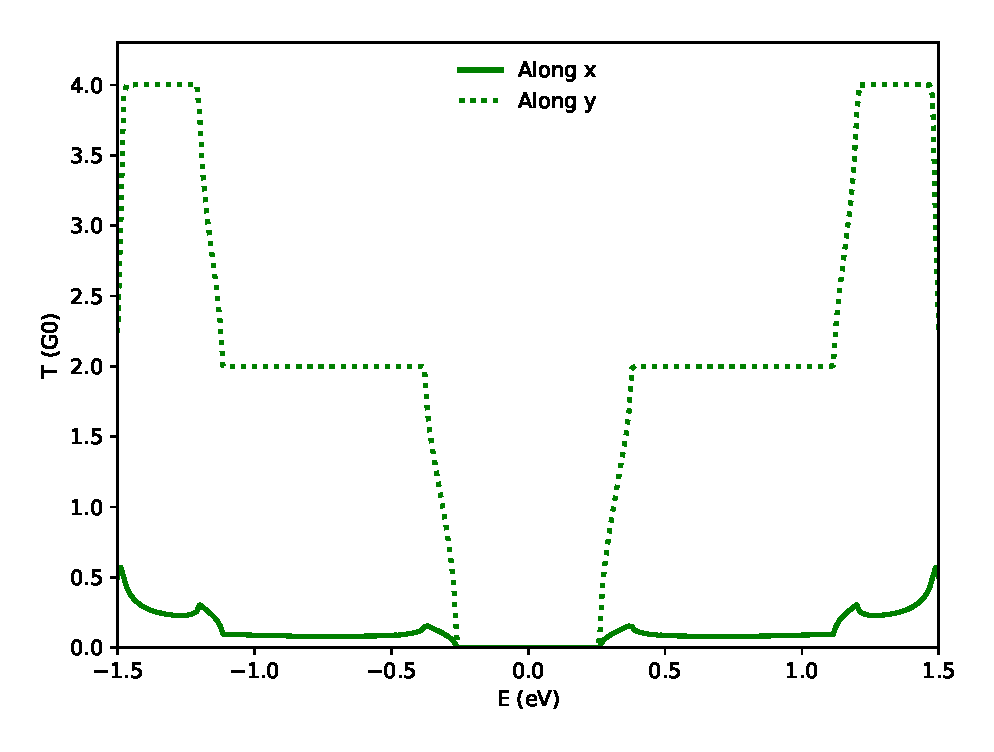
\includegraphics[width=0.35\textwidth]{Figures/txy_AVER.eps}
		\caption{Average over k-points \(0,\ \dfrac{\pi}{2},\ \pi \)}
		\label{piavg}
	\end{subfigure}
	\caption{Figure showing the comparison between plots of transmission through NPG obtained using the developed scripts (left/blue) and obtained using DFT (right/green).}\label{transmissionplots}
\end{figure}
As one can see in \cref{transmissionplots} The plots show very good correspondence with the DFT calculation. Again proving that the scripts developed on the basis of the tight-binding approximation can produce valid results, when it comes to band structure and transmission through NPG.\\
This concludes the preliminary work. The tools for calculation of band structures, LDOS and transmission has been successfully developed, using \textit{Python}-programming and the tight-binding approximation. Following will be a range of tests on different NPG systems, using the developed tools.
